\documentclass{article}
\usepackage[margin=1in]{geometry}
\usepackage{amsmath,amsthm,amssymb}
\usepackage{bbm,enumerate,mathtools}
\usepackage{tikz,pgfplots}
\usepackage{chessboard}
\usepackage[hidelinks]{hyperref}
\usepackage{multicol} % Problem 35

\newenvironment{question}{\begin{trivlist}\item[\textbf{Question.}]}{\end{trivlist}}
\newenvironment{note}{\begin{trivlist}\item[\textbf{Note.}]}{\end{trivlist}}
\newenvironment{references}{\begin{trivlist}\item[\textbf{References.}]}{\end{trivlist}}
\newenvironment{related}{\begin{trivlist}\item[\textbf{Related.}]\end{trivlist}\begin{enumerate}}{\end{enumerate}}


\begin{document}

\rating{3}{4}
The chromatic polynomial of a graph $G$, $\chi_G(n)$ gives the number of ways
to color the vertices of the graph such that no two vertices of the same color
are connected by an edge.

\begin{figure}[ht!]
  \centering
  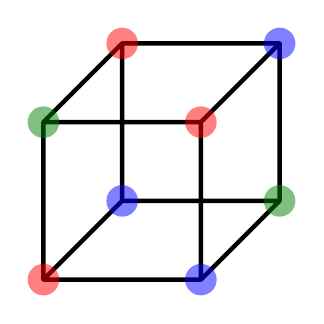
\begin{tikzpicture}
    \draw[ultra thick, line join=round]
      (1,3)--(3,3)--(2,2)--(0,2)--cycle
      (1,1)--(3,1)--(2,0)--(0,0)--cycle
      (0,0)--(0,2)
      (1,1)--(1,3)
      (2,0)--(2,2)
      (3,1)--(3,3);
    \fill[opacity=0.5, red]
      (0,0) circle (0.2)
      (2,2) circle (0.2)
      (1,3) circle (0.2);
    \fill[opacity=0.5, blue]
      (2,0) circle (0.2)
      (1,1) circle (0.2)
      (3,3) circle (0.2);
    \fill[opacity=0.5, green!50!black]
      (0,2) circle (0.2)
      (3,1) circle (0.2);
  \end{tikzpicture}
  ~
  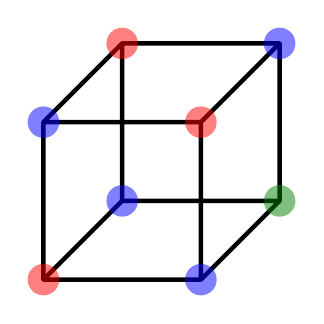
\begin{tikzpicture}
    \draw[ultra thick, line join=round]
      (1,3)--(3,3)--(2,2)--(0,2)--cycle
      (1,1)--(3,1)--(2,0)--(0,0)--cycle
      (0,0)--(0,2)
      (1,1)--(1,3)
      (2,0)--(2,2)
      (3,1)--(3,3);
    \fill[opacity = 0.5, red]
      (0,0) circle (0.2)
      (2,2) circle (0.2)
      (1,3) circle (0.2);
    \fill[opacity = 0.5, blue]
      (0,2) circle (0.2)
      (1,1) circle (0.2)
      (2,0) circle (0.2)
      (3,3) circle (0.2);
    \fill[opacity = 0.5, green!50!black]
      (3,1) circle (0.2);

  \end{tikzpicture}
  ~
  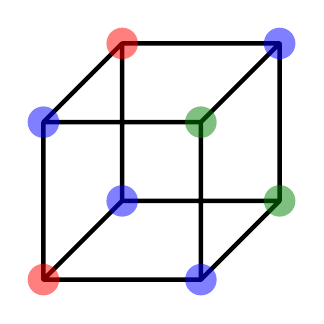
\begin{tikzpicture}
    \draw[ultra thick, line join=round]
      (1,3)--(3,3)--(2,2)--(0,2)--cycle
      (1,1)--(3,1)--(2,0)--(0,0)--cycle
      (0,0)--(0,2)
      (1,1)--(1,3)
      (2,0)--(2,2)
      (3,1)--(3,3);
    \fill[opacity=0.5, red]
      (0,0) circle (0.2)
      (1,3) circle (0.2);
    \fill[opacity=0.5, blue]
      (0,2) circle (0.2)
      (1,1) circle (0.2)
      (2,0) circle (0.2)
      (3,3) circle (0.2);
    \fill[opacity=0.5, green!50!black]
      (2,2) circle (0.2)
      (3,1) circle (0.2);
  \end{tikzpicture}
  \caption{Three examples of $3$-colorings of the cube. The chromatic polynomial
  of the cubic graph is ${\chi_{Q_3}(n) =
  a(n) = n^8 - 12n^7 + 66n^6 - 214n^5 + 441n^4 - 572n^3 + 423n^2 - 133n}$.}
\end{figure}

\begin{question}
  Is there a way to generate the chromatic polynomial of an $n$-cube in
  polynomial time with respect to $n$?
\end{question}

\begin{related}
  \item What about up to permutations of the colors and/or isometries of the cube?
  \item What about simplices, cross-polytopes, and demicubes?
  \item What about other polytopes such as associahedra, permutahedra, and
    the 24-, 120-, and 600-cells?
\end{related}

\begin{references}
  \item \url{https://math.stackexchange.com/q/3632156/121988}
  \item \url{https://oeis.org/A334230}
\end{references}
\end{document}
